Construct and sketch a joint 95\% confidence region for the mean difference vector $\bm{\delta}$
using the effluent data and results in Example 6.1. Note that the point $\bm{\delta} = \textbf{0}$ falls
outside the 95\% contour. Is this result consistent with the test of $H_{0}: \bm{\delta} = \textbf{0}$ considered
in Example 6.1? Explain.

\begin{figure}[H]
    \centering
    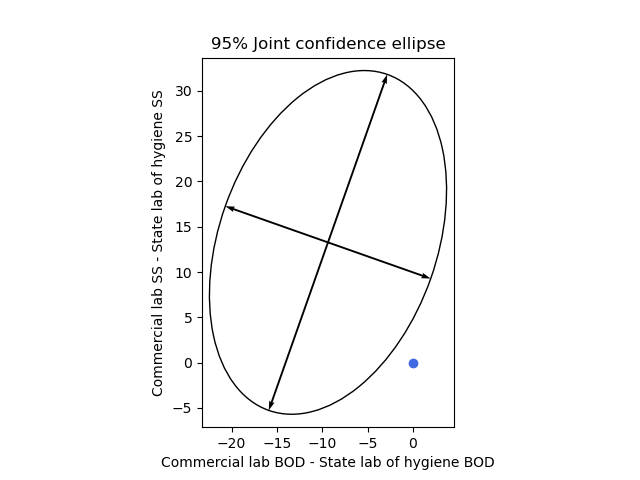
\includegraphics[scale=0.70]{./python/chapter-6/Question-6-1.png}
\end{figure}

Hoteling's $T^{2}$ tests $H_{0}: \bm{\delta}^{\prime} = [\delta_{1}, \delta_{2}] = [0, 0] = \textbf{0}^{\prime}$.
Basically,answering the question, is the vector $\textbf{0}$ inside the ellipse?
The conclusion was that the Hoteling's $T^{2}$ statistic of 13.6 was larger than the critical $F$ value of 9.47, so we rejected the null hypothesis $H_{0}$.
That is, the vector $\textbf{0}$ is not inside the ellipse. This is confirmed in the plot above, where the blue dot, $\textbf{0}$, is outside the ellipse.
The other conclusion was that the 95\% simultaneous confidence intervals for $\delta_{1}$ and $\delta_{2}$ did include 0.
This is also confirmed in the plot above, where if we project the ellipse onto each of the component axes we can see that the shadow it creates will include 0.